
\chapter{Introduction of Phishing}

While the Internet has brought convenience to many people for exchanging
information, it also provides opportunities to carry malicious behavior
such as online fraud on massive scale with a little cost to the attackers.
The attackers can manipulate the Internet users instead of computer
system (hardware or software) that significantly increase the barriers
of technological crime impact. Such human centered attack could be
done by social engineering. Phishing is a form of social engineering
that aim to retrieve credential from online users by mimicking trustworthy
and legitimate institutions \citep{jakobsson:2006}. These fraudulent
attacks are most frequently done by electronic communication such
as emails to direct users to fake websites and prompt for sensitive
information.

This chapter provides an overview to phishing modus operandi and its
current countermeasures such as detection and prevention techniques
along with a brief exploration of direct and indirect cost of phishing
attacks.


\section{What is phishing?}

In the real world, phishing has a similar basic principle as \textquoteleft fishing\textquoteright .
Instead of fish, online users are lured by authentic looking communication
and hooked by authentic looking websites. Phishing is a malicious
technique to manipulate online users into sharing their sensitive
information by masquerading as legitimate and trustworthy institutions.
Phishing attack also is a form of online criminal activity by using
social engineering technique \citep{jakobsson:2006}. An individual
or a group who uses this technique is called \emph{Phishers}. After
successfully gain sensitive information from the victim, phishers
use this information to access victim\textquoteright s financial accounts
or committing credit card frauds. The technique of phishing may vary,
but the most common technique of phishing attacks done by using fraudulent
emails and websites \citep{james:2005}. A fraudulent website is designed
in such a way that it would be very identical to its legitimate target.


\section{History of phishing}

The first time the term \textquotedbl{}phishing\textquotedbl{} was
published by the American Online (AOL) UseNet Newsgroup on January
2, 1996 and began to expand in 2004 \citep{phishorg}. Since then,
phishing development in cyberspace unfortunately was a great achievement
by phishers to make profit. Total losses due to phishing in 2004 reached
more than U.S. \$ 2 billion, it was involving more than 15,000 sites
that become victims \citep{fellman:2004}. Jakobsson, et al. mentioned
that in the early years of 90\textquoteright s (according to \citep{phishorg}
it was around 1995) many hackers would create bogus AOL user accounts
with automatically generated fraudulent credit card information \citep{jakobsson:2006}.
Their intention to give this fake credit card information was to simply
pass the validity tests performed by AOL. By the time the tests were
passed, AOL was thinking that these accounts were legitimate and resulted
to activate them. Consequently, these hackers could freely access
AOL resources until AOL tried to actually bill the credit card. AOL
realized that these accounts were using invalid billing information,
thus deactivated the account. 

While creating false AOL user accounts with fake credit card information
was not exactly phishing attacks, but AOL\textquoteright s effort
to counter against the attacks was leading to development of phishing.
This countermeasure includes directly verifying the legitimacy of
credit card information and the associated billing identity, forced
hackers to pursue alternative way \citep{jakobsson:2006}. Hackers
would masquerade themselves as AOL\textquoteright s employees asking
to other users for credit card information through AOL instant messenger
and email system. At this point, we believe the term of phishing attack
has been born. Since such attack has not been done before, many of
users have been victimized by then. Eventually, AOL enforced warning
system to the most of its customers to be vigilant when it comes to
sensitive information \citep{phishorg}. At the present day, phishing
attacks have evolved not only aim to AOL users, but also any online
users motivated by financial gain. Consequently, large number of legitimate
institutions such as PayPal and eBay are being spoofed.


\section{Formal definition of phishing}

Before we begin to dig deeper understanding of phishing attacks, we
will briefly explore common phishing definition. Currently, there
is no consensus definition, since almost in every research papers,
academic textbook or journals has its own definition of phishing \citep{jakobsson:2006,james:2005,tally:2004,clayton:2005,parno:2006,jakobsson:2005,dhamija:2006}.
Phishing is also constantly evolving, so it might be very challenging
to define its universal terminology. There is not so much study that
specifically addresses the standard of phishing definition. We will
take a look of one particular phishing definition from various sources:
\begin{enumerate}
\item Phishing is the act of sending a forged e-mail (using a bulk mailer)
to a recipient, falsely mimicking a legitimate establishment in an
attempt to scam the recipient into divulging private information such
as credit card numbers or bank account passwords \citep{james:2005}
\item Phishing is a form of Internet scam in which the attackers try to
trick consumers into divulging sensitive personal information. The
techniques usually involve fraudulent E-mail and web sites that impersonate
both legitimate E-mail and web sites \citep{tally:2004}
\item Phishing is an attack in which victims are lured by official looking
email to a fraudulent website that appears to be that of a legitimate
service provider \citep{clayton:2005}
\item In phishing, an automated form of social engineering, criminals use
the internet to fraudulently extract sensitive information from businesses
and individuals, often by impersonating legitimate web sites \citep{parno:2006}
\end{enumerate}
It is noteworthy that the definition described by {[}2, 5, 6{]} specifies
that the phishers only use email as a communication channel to trick
potential victims. While it might be true because using email would
greatly cost effective, but we believe that phishing is not only characterized
by one particular technological mean, as phishers can also use any
other electronic communication to trick potential victims (i.e private
message on online social network). This definition is also similar
to dictionary libraries {[}10-12{]} that mention email as a medium
communication between phishers and users.

We believe that standard definition of phishing should be applicable
in most of phishing concept that are presently defined. Consequently,
the high level of abstraction and is required to build common definition
on phishing. We also argued that the definition of phishing should
not focus on the technology being used but rather on the methodology
how the deception being conducted. Therefore, We follow the definition
of phishing by Lastdrager {[}13{]} which stated: 
\begin{quote}
\textit{Phishing is a scalable act of deception whereby impersonation
is used to obtain information from a target}
\end{quote}
The definition presented above is developed in a comprehensive way
by using existing definitions as input and combined them. A systematic
review of literature up to August 2013 was conducted along with manual
peer review, which resulted in 113 distinct definitions to be analyzed.
We thereby agree with Lastdrager {[}13{]} that this definition addresses
all the essential elements of phishing and we will adopt it as universally
accepted terminology throughout our research.


\section{Economics impact caused by phishing}

It is non-trivial task to find a real cost from phishing damage in
term of money or direct cost. This due to phishing economy is consistent
with black market economy and does not advertise its successes {[}1{]}.
On this section, brief explanation of direct cost on phishing attack
will be illustrated based on literature reviews.

The difficulty of assessing the damage on phishing attack is caused
by unwillingness of many users to share to acknowledge that they have
been victimized by phishing attacks. This happens might be because
of fear of humiliation, financial loses, or legal liability {[}1{]}.
However, studies estimate the damage ranging from \$61 million {[}14{]}
to \$3 billion per year {[}15{]} of direct losses to victims in the
US only {[}16{]}. The Gartner Group claimed to estimate of \$1.2 billion
direct losses of phishing attack to US banks and credit card companies
for the year 2004 {[}17{]}. By the 2007, it escalated to more than
\$3 billion loss {[}18{]}. The estimation also performed by TRUSTe
and Ponemon Institute that stated the cost of phishing attack was
up to \$500 millions losses in the US for the same year %
\footnote{http://www.theregister.co.uk/2004/09/29/phishing\_survey/%
}. Moreover, figure {[}num{]} illustrated the direct cost of phishing
in 2013 by the same companies. <still in progress> 


\section{Phishing modus operandi}

As we mentioned earlier, Phishing attack is a form of cybercrime.
The technique of the attack usually carried out firstly by creating
a replica/clone of a legitimate website such as financial website
with almost 100\% similar. After that, the phishers will try to trick
the potential victim to submit important information such as usernames,
passwords, PINs, etc. through a fake website that they have created.
With the information obtained, they will try to steal money from their
victims. Phishers employ variety of techniques to trick potential
victims to access their fraudulent website. One of the typical ways
is by sending illicit email in a large scale claiming to be from legitimate
institution. In the email content, they usually imitate an official-looking
logo, using good business language style and often also forge the
email headers to make it look like originating from legitimate institution.
Typically, the content of the email is to inform the user that the
bank is changing its IT infrastructure, and request urgently that
the customer should update their data with the consequence of loosing
their money if the action does not take place. When the user click
the link that was on the email message, they will be redirected to
a fraudulent website, which will prompt the victim to fill in the
details of their information. While there are various techniques of
phishing attack, we will address the common phases of phishing that
we are analyzed by literature survey and we will present our own phase. 

Based on the example scenario explained earlier, we believe that phishing
attacks may consist of several phases. J. Hong {[}16{]} argued that
there are three major phases:
\begin{enumerate}
\item Potential victims receive a phish.
\item The victim may take a suggested action in the message.
\item The phisher monetizes the stolen information.
\end{enumerate}
Frauenstein, et al. {[}19{]} suggested that typically there are five
main processes are used to perform phishing attack. On the first process,
a phisher usually will do some reconnaissance on how would the attack
is executed and what information would be obtained from the victim.
The first process is called planning. On the second process, a phisher
typically deliver its message via email. This email is desired by
the phisher to look as legit as possible to potential victim. For
this purpose, target institutions logo, trademark, symbol, etc. are
used to make the content look official to the victim. The author called
this process as Email Design. \autoref{fig:ing} illustrates the example
of fake ING bank logo in a phishing email to create \textquotedblleft legitimate\textquotedblright{}
feel%
\footnote{http://www.martijn-onderwater.nl/wp-content/uploads/2010/03/ing-phishing.jpg%
}.

\begin{figure}
\begin{centering}
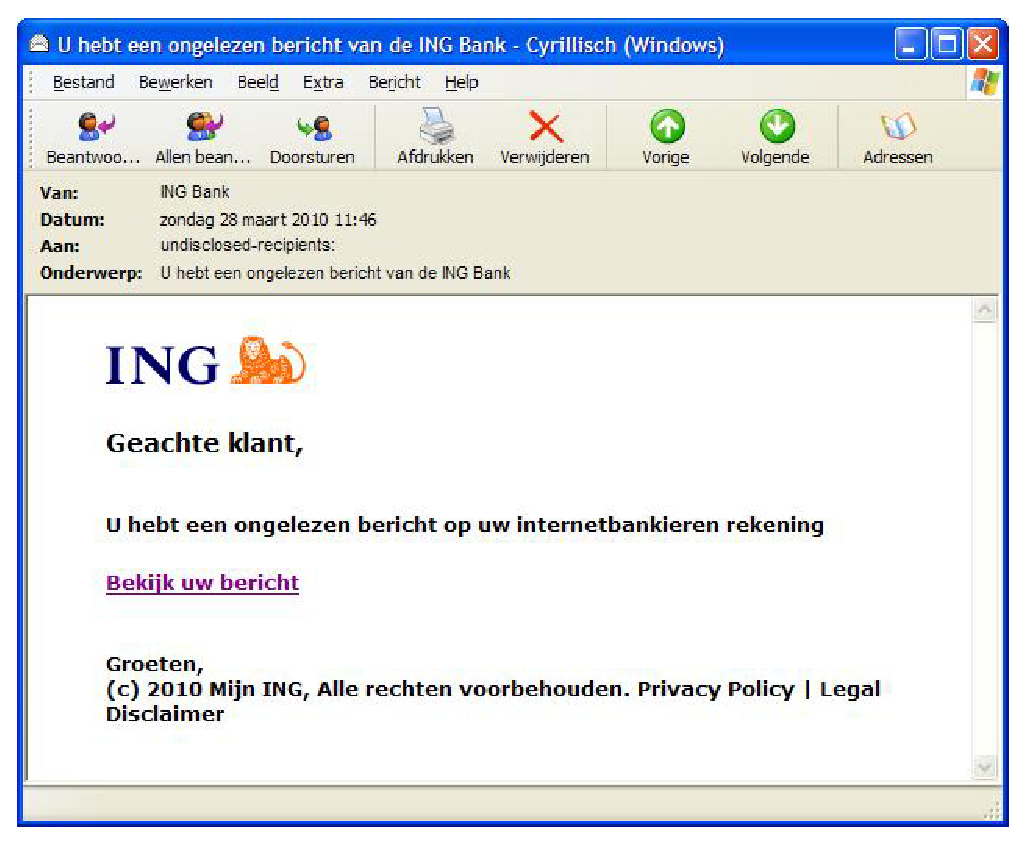
\includegraphics[scale=0.4]{gfx/ing-phishing}
\par\end{centering}

\protect\caption{\label{fig:ing}Example of fake ING logo in phishing email}
\end{figure}


On the third process, phisher fabricate a story to make potential
victim think that email is important. To achieve users attention,
usually phisher build up a story about system upgrade, account hijacked,
security enhancement, etc. so that the victim would feel obliged to
be informed. This technique is commonly known as reverse social engineering.
Moreover, we believe this process also corresponds with Cialdini {[}20{]}
that suggested reciprocation as one of the technique to persuade people.
On the fourth process, a phisher usually include threatening tone
or explain the urgency and consequences if the potential victim chooses
not to take action desired by the phisher (for example; account removal,
account blocked, etc.). Consequently, users may fear of their account
being deleted. This process also corresponds with the theory of persuasion
called authority {[}20{]}. The last process involved with fraudulent
website that has been created by the phisher. Users may falsely believe
to the message given in the email and may click a URL/link that is
embedded in the email. Subsequently, the URL would redirect users
to this fraudulent website that typically prompt users\textquoteright{}
sensitive information. Furthermore, the website is created to be as
similar as possible to the target institution\textquoteright s website,
so that potential victim may still believe that it is authentic. We
will explain more on Cialdini\textquoteright s six basic tendencies
of human behavior in generating positive response to persuasion {[}20{]}
in a later section. To make a better understanding, we have created
a diagram of these processes based on Frauenstein\textquoteright s
typical five main processes {[}19{]} in \autoref{fig:frauenstein}.

\begin{figure}
\begin{centering}
\includegraphics[scale=0.5]{\string"gfx/phishing processes\string".png}
\par\end{centering}

\protect\caption{\label{fig:frauenstein}Phishing processes based on Frauenstein\citep{frauenstein:2013}}


\end{figure}


Considering that phishing attack is a process, Wetzel {[}21{]} suggested
a taxonomy to make sense of the complex nature of the problem by mapping
out a common attack lifecycle, and a possible set of activities attackers
engage in within each phase. The taxonomy is illustrated in \autoref{fig:wetzel}.

\begin{figure}
\begin{centering}
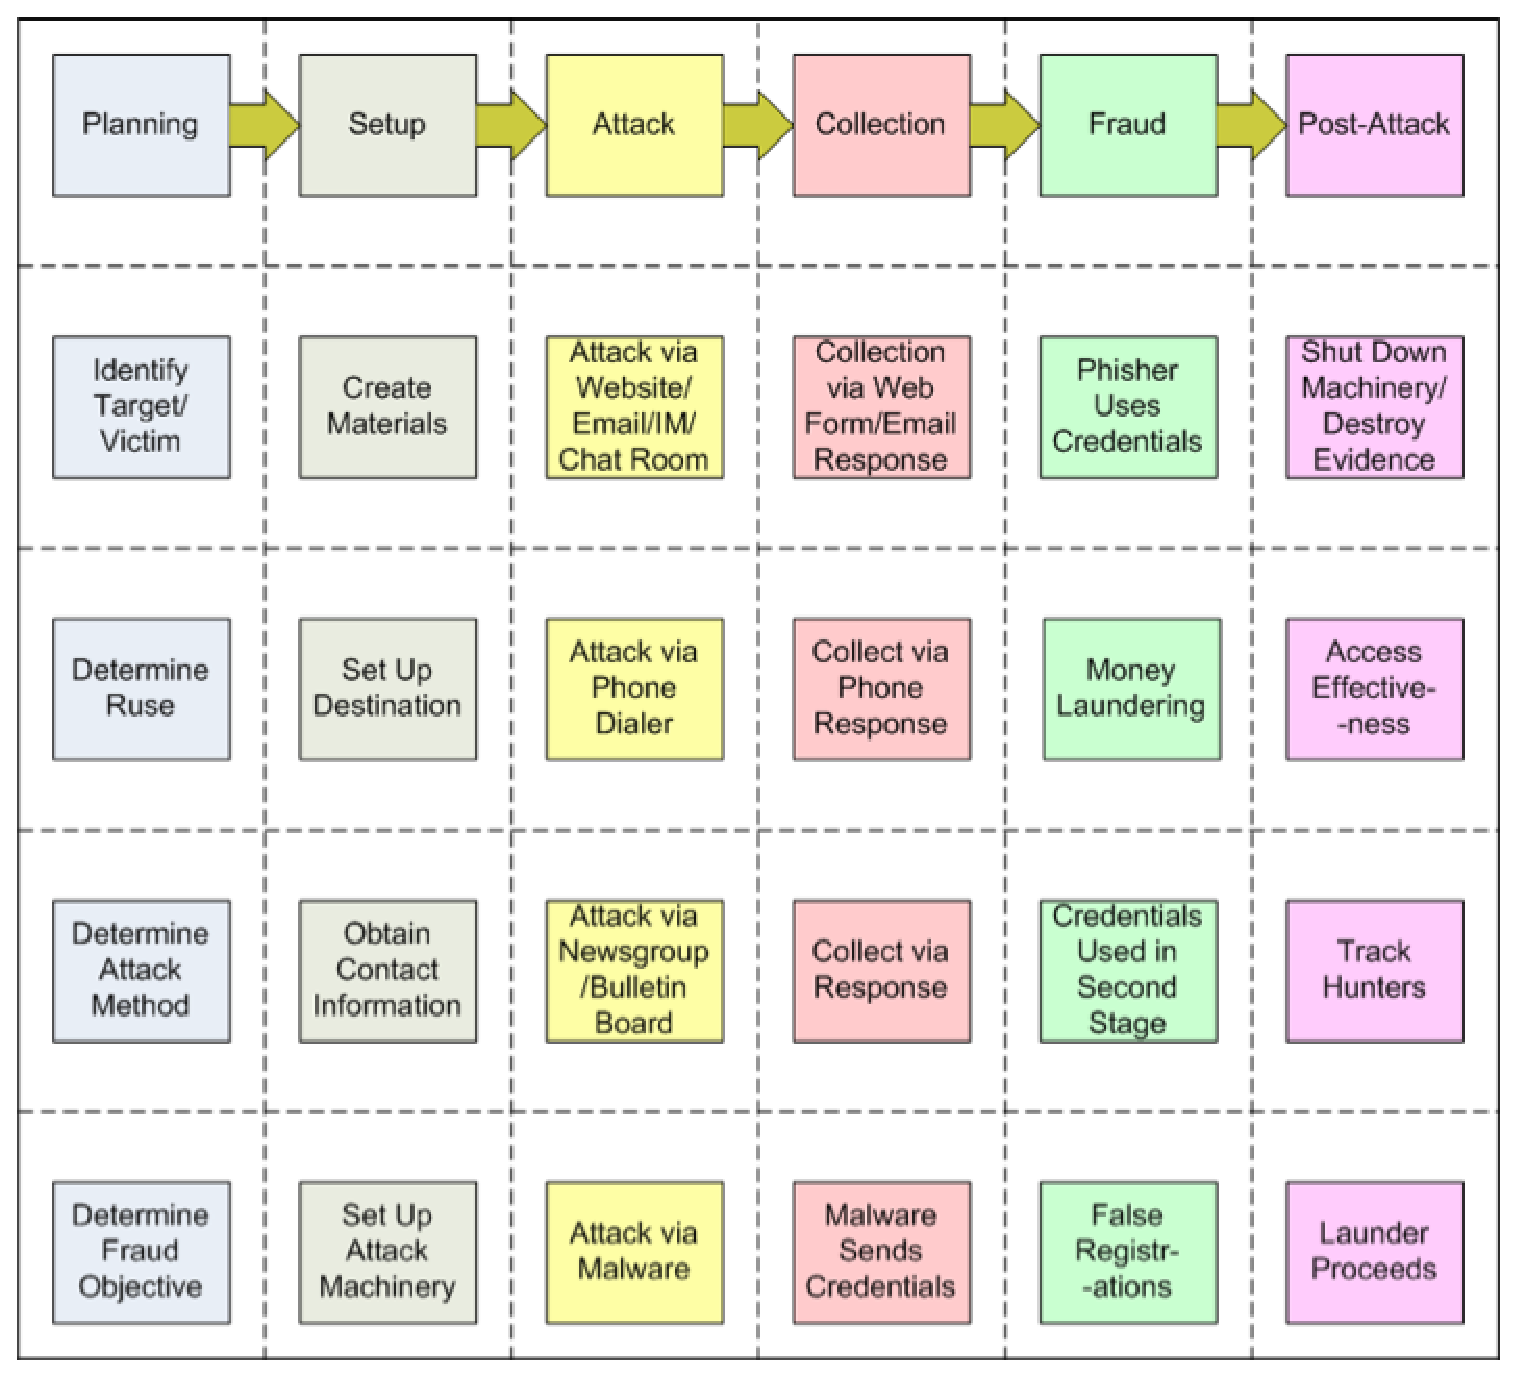
\includegraphics[scale=0.4]{gfx/wetzel}\protect\caption{\label{fig:wetzel}Phishing attack taxonomy and lifecycle\citep{wetzel:2005}}

\par\end{centering}

\end{figure}


A study suggest that there are several phases involved in phishing
attack {[}5{]}: 
\begin{enumerate}
\item The attacker obtains E-mail addresses for the intended victims. These
could be guessed or obtained from a variety of sources. 
\item The attacker generates an E-mail that appears legitimate and requests
the recipient to perform some action. 
\item The attacker sends the E-mail to the intended victims in a way that
appears legitimate and obscures the true source.
\item Depending on the content of the E-mail, the recipient opens a malicious
attachment, completes a form, or visits a web site. 
\item The attacker harvests the victim\textquoteright s sensitive information
and may exploit it in the future. 
\end{enumerate}
The phases described by {[}5{]} are also analogous with the information
flow explained by {[}22{]} represented in \autoref{fig:emigh}. 

\begin{figure}


\begin{centering}
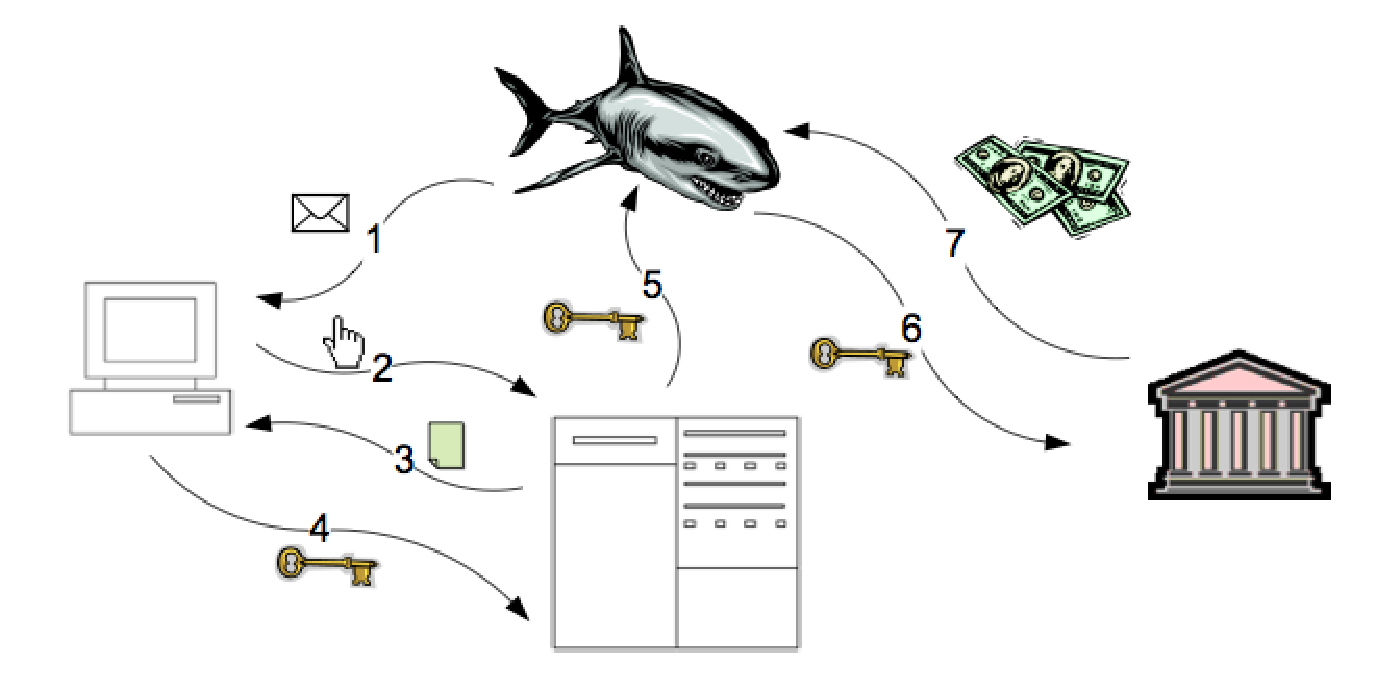
\includegraphics[scale=0.4]{gfx/emigh}\protect\caption{\label{fig:emigh}Flow of information in phishing attack \citep{emigh:2005}}

\par\end{centering}

\end{figure}


Quoted from Emigh {[}22{]}, the information flow of phishing attack
is described by the following phases without countermeasures part:
\begin{enumerate}
\item A malicious payload arrives through some propagation vector. 
\item The user takes an action that makes him or her vulnerable to an information
compromise. 
\item The user is prompted for confidential information, either by a remote
web site or locally by a Web Trojan. 
\item The user compromises confidential information. 
\item The confidential information is transmitted from a phishing server
to the phisher. 
\item The confidential information is used to impersonate the user. 
\item The phisher engages in fraud using the compromised information. 
\end{enumerate}
Phishing attack steps are also addressed by {[}23{]}. In their study,
a successful phishing attack involves several phases: 
\begin{enumerate}
\item Preparation 
\item Delivery of the Lure 
\item Taking the Bait 
\item Request for Confidential Information 
\item Submission of Information 
\item Collection of Data 
\item Impersonation 
\item Financial Gain
\end{enumerate}
As we can see from the earlier phases, there is a high amount of similarity
between each other. We believe our phases are also analogous with
other earlier studies. We thereby present our own phases of phishing
attack and its categorization such as the lure, the hook and the catch.
From \autoref{fig:Information-flow-phishing}, we believe that the
phishers generally characterized in the following way:
\begin{itemize}
\item The lure \end{itemize}
\begin{enumerate}
\item Phishers prepare the attack 
\item Deliver initial payload to victim 
\item Direct spoofed website \end{enumerate}
\begin{itemize}
\item The hook \end{itemize}
\begin{enumerate}[resume]
\item Prompt for confidential information
\item Disclosed confidential information 
\item Collect stolen information \end{enumerate}
\begin{itemize}
\item The catch\end{itemize}
\begin{enumerate}[resume]
\item Impersonates victim 
\item Received pay out from the bank 
\end{enumerate}
\begin{figure}
\centering{}\includegraphics[scale=0.3]{gfx/info-flow-nolie}\protect\caption{\label{fig:Information-flow-phishing}Information flow phishing attack}
\end{figure}



\section{Common type of phishing}

In January 2014, 8300 patients data are being compromised in medical
company in the US%
\footnote{http://www.scmagazine.com/medical-staffers-fall-for-phishing-emails-data-on-8300-compromised/article/340590/%
}. The data includes names, addresses, date of birth and phone numbers
were being stolen. Other than demographic information, clinical information
associated with this data was also stolen, including social security
numbers. In the April 2014, phisher has successfully stole US\$163,000
from US public school based on Michigan%
\footnote{http://www.scmagazine.com/phishing-scam-targets-michigan-public-schools/article/343177/%
}. It has been said that the email prompted to transfer money is coming
from the finance director of the school. In March 2014, Symantec has
discovered phishing attack aimed at Google drive users%
\footnote{http://www.scmagazine.com/phishing-scam-aimed-at-google-docs-drive-users/article/338369/%
}. The attack was carried firstly with incoming email asking for opening
document hosted at Google docs. Users that have clicked on the link
are taken to fraudulent Google login page prompted Google users credentials.
Interestingly, the URL seems very convincing because it hosted on
Google secure servers. We believe even more phishing incidents on
financial area as well, but sometimes the news is kept hidden due
to creditability reason.

One may ask, what type of phishing are these? What type of phishing
commonly used nowadays? The threat of phishing attacks is still alarming
until today, and will be evolving in the future with more sophisticated
technique of attacks. For this reason, we believe that it is necessary
to provide a brief insight on popular variants of phishing that currently
exist. 


\subsection{Deceptive phishing}

There are many variations based on deceptive phishing schemes. Typical
scenario of deceptive phishing schemes is to send a large amount of
illicit emails containing call to action asking recipients to click
embedded links {[}1{]}. These variations include cousin domain attack.
For example, legitimate PayPal website addressed as www.paypal.com,
this cousin domain attacks confuse potential victims to believe that
www.paypal-security.com is a subdivision of the legitimate website
due to identical looking addresses. Similarly, homograph attacks create
a confusion using similar characters to its addresses. For example,
www.paypal.com and www.paypa1.com, both addresses look the same but
on the second link, it uses \textquotedblleft 1\textquotedblright{}
instead of \textquotedblleft l\textquotedblright . 

Moreover, phishers may embed a login page directly to the email content.
This suggests the elimination of the need of end-users to click on
a link and phishers do not have to manage an active fraudulent website.
IP addresses are often used instead of human readable hostname to
redirect potential victim to phishing website and JavaScript is used
to take over address bar of a browser to make potential victims believe
that they are communicating with the legitimate institution. We will
also see few examples of malicious JavaScript on our preliminary analysis
section. 

Another type of deceptive phishing scheme is rock-phish attacks. They
held responsible for half a number of reported incidents worldwide
in 2005 {[}24{]}. These attacks evade email filters by utilizes random
text and GIF images which contain the actual message. Rock phish attacks
also utilize a toolkit that capable to manage several fraudulent websites
in a single domain. Sometimes, deceptive phishing schemes lead to
installation of malware when users visit fraudulent website and we
will describe malware based phishing scheme in the next section. 


\subsection{Malware-based phishing}

Generally, malware based phishing refers to any type of phishing which
involves installing malicious piece of software onto users' personal
computer {[}1{]}. Subsequently, this malware is used to gather confidential
information from victims instead of spoofing legitimate websites.
This type of phishing incorporates malwares such as keyloggers/screenloggers,
web Trojans and hosts file poisoning.


\subsection{Man in the middle phishing}

\begin{figure}


\centering{}\includegraphics[scale=0.4]{gfx/jakobsson}\protect\caption{\label{fig:jakobsson}Man in the middle phishing\citep{jakobsson:2006}}
\end{figure}


Man-in-the-middle phishing attacks refer to the phishers that positioned
in the middle between a legitimate institution and an end user {[}1{]}.
The objective of these attacks is to make end users and legitimate
institution (eg. Internet banking website) believe that they are truly
communicating with each other. According to {[}1{]}, \autoref{fig:jakobsson}
illustrates the information flow of this type of attacks. Confidential
information intended for legitimate site will be passed to the phishers
before they can forward it to the legitimate site. Similarly, information
from legitimate site to end-users will be passed to the phishers first
before the phishers can forward it to them. Unfortunately, man-in-the-middle
attacks are also capable to exploit two-factor authentication system
(sometimes called two steps verification) that ensures the authenticity
of sender and recipient (Eg. Popular ABN Amro case in 2007%
\footnote{http://www.theregister.co.uk/2007/04/19/phishing\_evades\_two-factor\_authentication%
}).


\section{Bad neighborhoods on phishing}

In the real world, there are parts of certain area that have higher
crime rates than others (eg. Bronx in the US). Evidently, it is statistically
more likely that a crime will occur compared to other locations {[}25{]}.
To better illustrate this analogy, the police department in Belgium%
\footnote{http://www.polfed-fedpol.be/%
} has put up statistical information regarding crime rates in the country.
\autoref{fig:car-incidents} shows an example in 2013; there were
up to 5525 car theft incidents recorded and we can see there are certain
areas that have higher probability that a car got stolen. For example,
Antwerp had 415 incidents whereas Berlare had only 1 car theft incident%
\footnote{http://www.polfed-fedpol.be/crim/crim\_statistieken/ app\_crimestat/app\_crimestat\_dashboard\_crimfig\_misdrijven\_nl.php%
}. The data is not necessarily based on cities, it can be based on
the residential area within a city. This holds true that much higher
crime rates in a concentrated location compared to any other locations.
It is called bad neighborhood. 

\begin{figure}


\begin{centering}
\includegraphics[scale=0.8]{\string"gfx/bad neighborhoods\string".png}\protect\caption{\label{fig:car-incidents}Belgium police record on car theft incidents
in 2013}

\par\end{centering}

\end{figure}


To reduce the crime rates in a bad neighborhood, it makes sense that
the authority should put more enforcement in this location. Moreover,
the citizen should avoid this location as much as they can if they
want to feel much safer. Evidently, the existence of bad neighborhood
phenomenon also occurs in the Internet world called ``Internet bad
neighborhoods''. There are certain networks of Internet infrastructure
that contain more malicious activities that other networks. For our
preliminary analysis, we will adopt formal definition of Internet
bad neighborhoods or Internet Badhoods by {[}25{]} which states: 
\begin{quote}
\textit{Internet bad neighborhood is a set of IP addresses clustered
according to an aggregation criterion in which a number of IP addresses
perform a certain malicious activity over a specified period of time}
\end{quote}
Several studies have suggested that the source of the Internet Badhoods
tend to be concentrated in certain portions of IP address space {[}26-28{]}.
A dissertation study argues that Internet Badhoods do not always only
based on network prefixes level (e.g. /24, /32, etc..) but it can
be aggregated into several levels (ISPs, Countries) {[}25{]}. Moreover,
Internet Badhoods may vary depending on which application exploited.
While spam is most likely distributed all around the world, however,
phishing Badhoods are most likely concentrated in developed countries
(e.g. US) {[}25{]}. This suggests that phishing sites are required
to have more reliable hosts in term of availability, while spams are
not. We will see on section {[}num{]} our preliminary analysis on
phishing Badhoods.


\section{Current countermeasures of phishing attacks}

There are various types of phishing countermeasures. However, since
all the approaches reviewed so far all are preventive in nature, we
believe phishing detection also aims to prevent user\textquoteright s
confidential information to be successfully transmitted onto the wrong
hands. A study suggests that phishing detection can be classified
into two types; user training approach and software classification
approach {[}29{]}. \autoref{fig:Phishing-detection} categorizes the
current countermeasures that presently developed. \autoref{tab:adv-dis}
also indicates the advantages and the disadvantages of each category\citep{parmar:2014}.
However, we do not aim to give a complete wide range literature survey
on all available phishing countermeasures. We also do not evaluate
the effectiveness of current anti-phishing technology. We will only
discuss our result of literature review on Phishtank as a blacklist
and machine learning classification, and anti-phishing training as
prevention.

\begin{figure}


\begin{centering}
\includegraphics[scale=0.8]{gfx/countermeasures}\protect\caption{\label{fig:Phishing-detection}Phishing detection\citep{parmar:2014}}

\par\end{centering}

\end{figure}


\begin{table}
\begin{tabular}{>{\raggedright}p{2cm}>{\raggedright}p{4cm}>{\raggedright}p{4cm}}
\toprule 
\textbf{\footnotesize{}Detection techniques} & \textbf{\footnotesize{}Advantages} & \textbf{\footnotesize{}Disadvantages}\tabularnewline
\midrule 
{\scriptsize{}Blacklist} & \begin{itemize}
\item {\scriptsize{}Requiring low resources on host machine }{\scriptsize \par}
\item {\scriptsize{}Effective when minimal FP rates are required }\end{itemize}
 & \begin{itemize}
\item {\scriptsize{}Mitigation of zero hour phishing attack }{\scriptsize \par}
\item {\scriptsize{}Can result in excessive queries with heavily loaded
servers }\end{itemize}
\tabularnewline
\midrule 
{\scriptsize{}Heuristics and visual similarity} & \begin{itemize}
\item {\scriptsize{}Mitigate zero hour attacks}\end{itemize}
 & \begin{itemize}
\item {\scriptsize{}Higher FP rate than blacklists}{\scriptsize \par}
\item {\scriptsize{}High computational cost }\end{itemize}
\tabularnewline
\midrule 
{\scriptsize{}Machine Learning} & \begin{itemize}
\item {\scriptsize{}Mitigate zero hour attacks}{\scriptsize \par}
\item {\scriptsize{}Construct own classification model }\end{itemize}
 & \begin{itemize}
\item {\scriptsize{}Time consuming}{\scriptsize \par}
\item {\scriptsize{}Costly}{\scriptsize \par}
\item {\scriptsize{}Huge number of rules }\end{itemize}
\tabularnewline
\bottomrule
\end{tabular}\protect\caption{\label{tab:adv-dis}Advantages-disadvantages detection technique\citep{parmar:2014}}


\end{table}



\subsection{Phishing detection}


\subsubsection{Phishtank}

One of the common approaches to detect phishing attack is blacklisting.
Phishtank is a blacklisting company specifically for phishing URLs
and it is a free community web based where users can report, verify
and track phishing URLs. Phishtank stores phishing URLs in its database
and the data is widely available for use by other companies. Some
of the big companies that are using Phishtank\textquoteright s data
includes; Yahoo Mail, McAfee, APWG, Web Of Trust, Kaspersky, Opera
and Avira. In this section, we will discuss how the current literatures
have to do with the data provided by Phishtank. \autoref{tab:phishtank}
summarizes the papers selected and its relevancy with Phishtank.

\begin{longtable}{>{\raggedright}p{3cm}>{\raggedright}p{2cm}>{\raggedright}p{2cm}>{\raggedright}p{5cm}}
\caption{\label{tab:phishtank}Summary phishtank studies}
\tabularnewline
\toprule 
\textbf{\footnotesize{}Paper title} & \textbf{\footnotesize{}First author} & \textbf{\footnotesize{}Country} & \textbf{\footnotesize{}Relevancy with phishtank}\tabularnewline
\midrule 
{\scriptsize{}Evaluating the wisdom of crowds in assessing phishing
website {[}30{]}} & {\scriptsize{}Tyler Moore} & {\scriptsize{}United Kingdom} & {\scriptsize{}Examine the structure and outcomes of user participation
in Phishtank. The authors find that Phishtank is dominated by the
most active users, and that participation follows a power law distribution
and this makes it particularly susceptible to manipulation.}\tabularnewline
\midrule 
{\scriptsize{}Re-evaluating the wisdom of crowds in assessing web
Security {[}31{]}} & {\scriptsize{}Pern Hui Chia} & {\scriptsize{}Norway} & {\scriptsize{}Examine the wisdom of crowds on web of trust that has
similarity with Phishtank as a user based system.}\tabularnewline
\midrule 
{\scriptsize{}Automatic detection of phishing target from phishing
webpage {[}32{]}} & {\scriptsize{}Gang Liu} & {\scriptsize{}China} & {\scriptsize{}Phishtank database is used to test the phishing target
identification accuracy of their method.}\tabularnewline
\midrule 
{\scriptsize{}A method for the automated detection of phishing websites
through both site characteristics and image analysis {[}33{]}} & {\scriptsize{}Joshua S. White} & {\scriptsize{}New york, US.} & {\scriptsize{}Phishtank database is used to perform additional validation
of their method. They also collect data from twitter using twitter\textquoteright s
API to find malicious tweets containing phishing URLs}\tabularnewline
\midrule 
{\scriptsize{}Intelligent phishing detection and protection scheme
for online transaction {[}34{]} } & {\scriptsize{}P.A. Barraclough} & {\scriptsize{}Newcastle, United Kingdom} & {\scriptsize{}Phishtank features is used as one of the input of neuro
fuzzy technique to detect phishing website. The study suggested 72
features from Phishtank by exploring journal papers and 200 phishing
website.}\tabularnewline
\midrule 
{\scriptsize{}Towards preventing QR code based attacks on android
phone using security warning {[}35{]}} & {\scriptsize{}Huiping Yao} & {\scriptsize{}New Mexico, US.} & {\scriptsize{}Phishtank API is used for lookup whether the given QR
containing phishing URL in the Phishtank database.}\tabularnewline
\midrule 
{\scriptsize{}A SVM based technique to detect phishing URLs {[}36{]}} & {\scriptsize{}Huajun Huang} & {\scriptsize{}China} & {\scriptsize{}Phishtank database is used as validation resulting 99\%
accuracy by SVM method, plus the top ten brand names in Phishtank
archive is used as features in SVM method.}\tabularnewline
\midrule 
{\scriptsize{}Socio technological phishing prevention {[}37{]}} & {\scriptsize{}Gaurav Gupta} & {\scriptsize{}Australia} & {\scriptsize{}Analyze the Phishtank verifiers (individual/organization)
to be used as anti phishing model.}\tabularnewline
\midrule 
{\scriptsize{}An evaluation of lightweight classification methods
for identifying malicious URLs {[}38{]}} & {\scriptsize{}Shaun Egan} & {\scriptsize{}Grahamstown, South Africa} & {\scriptsize{}Indicating that lightweight classification methods achieves
an accuracy of 93\% to 96\% when trained data from Phishtank.}\tabularnewline
\midrule 
{\scriptsize{}Phi.sh/\$oCiaL: The phishing landscape through short
URLs {[}39{]}} & {\scriptsize{}Sidharth Chhabra} & {\scriptsize{}Delhi, India} & {\scriptsize{}Phishtank database is used to analyze suspected phish
that is done through short URLs.}\tabularnewline
\midrule 
{\scriptsize{}Discovering phishing target based on semantic link network
{[}40{]}} & {\scriptsize{}Liu Wenyin} & {\scriptsize{}Hong Kong} & {\scriptsize{}Phishtank database is used as test dataset to verify
their proposed method (Semantic Link Network) }\tabularnewline
\end{longtable}

From our literature survey, we know that Phishtank is crowd-sourced
platform to manage phishing URL, for that reason a study aims to evaluate
the wisdom of crowd provided by Phishtank {[}30{]}. The study finds
that the user participation is distributed according to power law.
It uses to model data which frequency of an event varies as a power
of some attribute of that event {[}41{]}. However, according to {[}42{]},
quantifying power law distribution by approximately straight-line
behavior should not be trusted. However, while it may be true, it
makes sense that in Phishtank\textquoteright s verification system,
a single highly active user\textquoteright s action can greatly impact
the system\textquoteright s overall accuracy. \autoref{tab:Comparison-summary}
summarizes the comparison performed by {[}30{]} between Phishtank
and closed proprietary anti-phishing feeds%
\footnote{The author did not specify the identity of the closed proprietary
company%
}. Moreover, there are some ways to disrupt Phishtank verification
system; submitting invalid reports accusing legitimate website, voting
legitimate website as phish, and voting illegitimate website as not
phish. While the last action is obviously for phisher\textquoteright s
benefit, the first two actions rather subtle intention to undermine
Phishtank credibility.

To put it briefly, the lesson of crowd sourced anti-phishing technology
like Phishtank is that the distribution of user participation matters.
It means that if a few high value participants do something wrong,
it can greatly impact overall system. Also, there is a high probability
that bad users could also extensively participate in submitting or
verifying URLs in Phishtank, which is unacceptable. 

\begin{table}


\begin{tabular}{>{\centering}p{4cm}>{\centering}p{3cm}}
\toprule 
\textbf{\footnotesize{}Phishtank} & \textbf{\footnotesize{}Proprietary}\tabularnewline
\midrule
\midrule 
{\scriptsize{}10924 URLs} & {\scriptsize{}13318 URLs}\tabularnewline
\midrule 
{\scriptsize{}8296 URLs after removing duplication} & {\scriptsize{}8730 URLs after removing duplication}\tabularnewline
\midrule 
\multicolumn{2}{c}{{\scriptsize{}Shares 5711 URLs in common 3019 Unique to the company
feeds while 2585 only appeared in Phishtank}}\tabularnewline
\midrule 
{\scriptsize{}586 rock-phish domains} & {\scriptsize{}1003 rock phish domains}\tabularnewline
\midrule 
{\scriptsize{}459 rock phish domains found in Phishtank} & {\scriptsize{}544 rock phish domains not found in Phishtank}\tabularnewline
\midrule 
{\scriptsize{}Saw the submission first} & {\scriptsize{}11 minutes later appear on the feed}\tabularnewline
\midrule 
{\scriptsize{}16 hours later after its submission for verification
(voting based)} & {\scriptsize{}8 second to verified after it appears}\tabularnewline
\midrule 
{\scriptsize{}Rock phish appear after 12 hours appeared in the proprietary
feed and were not verified for another 12 hours} & \tabularnewline
\bottomrule
\end{tabular}\protect\caption{\label{tab:Comparison-summary}Comparison summary}


\end{table}



\subsubsection{Machine learning approach}

The fundamental of phishing detection system would be to distinguish
between phishing websites and the legitimate ones. As we previously
discussed, the aim of phishing attack is to gather confidential information
from potential victims. To do this, phishers often prompt for this
information through fraudulent websites and masquerade as legitimate
institutions. It does not make sense if phishers created them in a
way very distinctive with its target. It may raise suspicions with
result of unsuccessful attack. To put it another way, most of the
phishing websites are mostly identical with its legitimate websites
as target to reduce suspiciousness from potential victim. 

In contrast of blacklisting technique that heavily depend on human
verification, researchers make use of machine learning based technique
to automatically distinguish between phishing and legitimate either
websites or email. Basically, machine-learning system is a platform
that can learn from previous data and predict future data with its
classification, in this case, phishing and legitimate. In order for
this machine to learn from data, there should be some kind of inputs
to classify the data, it is called features or characteristics. 

Furthermore, there are also several learning algorithms to classify
the data, such as, logistic regression, random forest, neural networks,
support vector machine, etc.. However, we will not discuss about the
learning algorithm currently implemented. We will only introduce the
common features that are used in machine learning based detection. 

There are vast amount of features to utilize machine learning to detect
phishing attack. The most common features are lexical feature, host-based
feature and site popularity feature. Each of these features will be
introduced briefly in the following section. 


\subsubsection{Lexical features}

Lexical features (URL based features) are based on the analysis of
URL structure without any external information. A study suggest that
the structure URL of phishing may \textquotedblleft looks\textquotedblright{}
different to experts {[}43{]}. These features include how many dots
exist, the length, how deep the path traversal do the URL has, if
there any sensitive words present in a URL, etc.. For example the
URLs https://www.paypal.com and http://www.paypal.com.freehosting.com/
or http://login.freehosting.com/ www.paypal.com/, we can see that
the domain paypal.com positioned differently, with the first one being
the benign URL. \autoref{fig:ex-lex} shows the example analysis of
lexical features in a phishing URL {[}44{]}.

\begin{figure}


\centering{}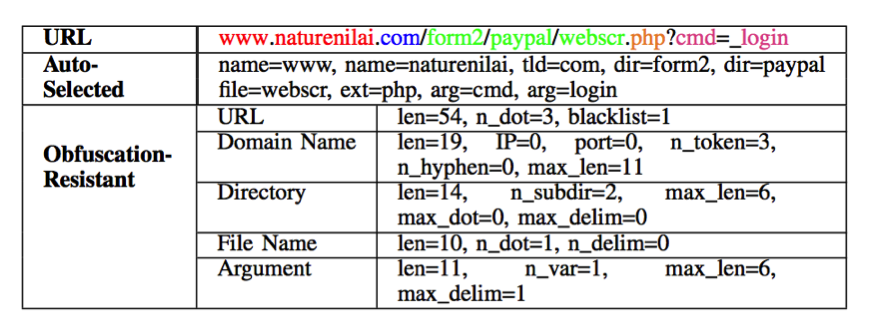
\includegraphics[scale=0.8]{gfx/lexical}\protect\caption{\label{fig:ex-lex}Example lexical features}
\end{figure}


We believe lexical features analysis has a performance advantage and
reduces overhead in term of processing and latency, since it only
tells the machine to learn URL structure. 90\% accuracy is achieved
when utilizing lexical features combined with external features such
as WHOIS data {[}44{]}. A study also performed evaluation of lightweight
classification that includes lexical features and host based features
in its model {[}38{]}. The study found that the classification based
on these features resulted in extremely high accuracy and low overhead.
\autoref{tab:exist-lex} lists the existing lexical features that
are currently implemented by two different studies {[}45, 46{]}. However,
{[}45{]} pointed out that URLs structure could be manipulated with
little cost, causing the features to fail. For example, attackers
could simply remove embedded domain and sensitive words to make their
phishing URLs look legitimate. There are also plenty of legitimate
domains presented only with IP address and contains more dots. Nevertheless,
lexical analysis would be suitable features to use for first phase
analysis in a large data {[}38{]}.

\begin{table}
\begin{tabular}{>{\raggedright}p{5cm}>{\raggedright}p{4cm}}
\toprule 
\textbf{\footnotesize{}Feature {[}46{]}} & \textbf{\footnotesize{}Feature {[}45{]}}\tabularnewline
\midrule
\midrule 
\begin{itemize}
\item {\scriptsize{}Length of hostname Length of entire URL}{\scriptsize \par}
\item {\scriptsize{}Number of dots Top-level domain}{\scriptsize \par}
\item {\scriptsize{}Domain token count}{\scriptsize \par}
\item {\scriptsize{}Path token count}{\scriptsize \par}
\item {\scriptsize{}Average domain token length}{\scriptsize \par}
\item {\scriptsize{}Average path token length}{\scriptsize \par}
\item {\scriptsize{}Longest domain token length}{\scriptsize \par}
\item {\scriptsize{}Longest path token length}{\scriptsize \par}
\item {\scriptsize{}Brand name presence }{\scriptsize \par}
\item {\scriptsize{}IP address presence}{\scriptsize \par}
\item {\scriptsize{}Security sensitive word presence }\end{itemize}
 & \begin{itemize}
\item {\scriptsize{}Embedded domain}{\scriptsize \par}
\item {\scriptsize{}IP address}{\scriptsize \par}
\item {\scriptsize{}Number of dots in URL}{\scriptsize \par}
\item {\scriptsize{}Suspicious URL }{\scriptsize \par}
\item {\scriptsize{}Number of sensitive words in URL}{\scriptsize \par}
\item {\scriptsize{}Out of position top level domain (TLD) }\end{itemize}
\tabularnewline
\bottomrule
\end{tabular}\protect\caption{\label{tab:exist-lex}Existing lexical features}
\end{table}



\subsubsection{Host based features}

Since phishers often hosted phishing websites in less reputable hosting
services and registrars, host-based features are needed to observe
on the external sources (WHOIS information, domain information, etc.).
A study suggests host-based features have the ability to describe
where phishing websites are hosted, who owns them and how they are
managed {[}43{]}. \autoref{tab:host-based} shows the host-based features
from two studies that are currently used in machine learning phishing
detection. 

\begin{table}
\begin{tabular}{>{\raggedright}p{3cm}>{\raggedright}p{5cm}>{\raggedright}p{3cm}}
\toprule 
\textbf{\footnotesize{}Justin Ma, et al.{[}43, 47{]}} & \textbf{\footnotesize{}Haotian Lio, et al.{[}46{]}} & \textbf{\footnotesize{}Guang Xiang, et al.{[}45{]}}\tabularnewline
\midrule
\midrule 
\begin{itemize}
\item {\scriptsize{}WHOIS data}{\scriptsize \par}
\item {\scriptsize{}IP address information}{\scriptsize \par}
\item {\scriptsize{}Connection speed}{\scriptsize \par}
\item {\scriptsize{}Domain name properties }\end{itemize}
 & \begin{itemize}
\item {\scriptsize{}Autonomous system number }{\scriptsize \par}
\item {\scriptsize{}IP country}{\scriptsize \par}
\item {\scriptsize{}Number of registration information}{\scriptsize \par}
\item {\scriptsize{}Number of resolved IPs}{\scriptsize \par}
\item {\scriptsize{}Domain contains valid PTR record}{\scriptsize \par}
\item {\scriptsize{}Redirect to new site}{\scriptsize \par}
\item {\scriptsize{}All IPs are consistent}\end{itemize}
 & \begin{itemize}
\item {\scriptsize{}Age of Domain}\end{itemize}
\tabularnewline
\bottomrule
\end{tabular}\protect\caption{\label{tab:host-based}Host-based features}
\end{table}


Each of these features does matter for phishing detection. However,
we will not describe each of these features in detail. It is noteworthy
that some of the features are subset of another feature, for instance,
autonomous system number (ASN), IP country and number of registration
information are derived from WHOIS information. Nevertheless, we will
only explain few of them that we believe the most crucial. 
\begin{enumerate}
\item WHOIS information: Since phishing websites are often created at relatively
young age, this information could provide the registration date, update
date and expiration date. Domain ownership would also be included;
therefore, a set of malicious websites with the same individual could
be identified. 
\item IP address information: Justin Ma, et al. used this information for
identify whether or not an IP address is in blacklist. Besides the
corresponding IP address, it provides records like nameservers and
mail exchange servers. This allows the classifier to be able to flag
other IP addresses within the same IP prefix and ASN. 
\item Domain name properties: these include time to live (TTL) of DNS associated
with a hostname. PTR record (reverse DNS lookup) of a domain could
also be derived whether it is valid or not.
\end{enumerate}
During our preliminary analysis, we will show that we could add reverse
IP address lookup to find bad neighborhoods within the same IP address
or domain. 


\subsubsection{Site popularity features}

Site popularity could be an indicator whether a website is phishy
or not. It makes sense if a phishing website has much less traffic
or popularity than a legitimate website. According to {[}45{]}, some
of the features indicated in \autoref{tab:popular-features} are well
performed when incorporated with machine learning system. 

\begin{table}
\begin{tabular}{>{\raggedright}p{5cm}>{\raggedright}p{3cm}}
\toprule 
\textbf{\footnotesize{}Guang Xiang, et al. {[}45{]}} & \textbf{\footnotesize{}Haotian Liu, et al. {[}46{]}}\tabularnewline
\midrule
\midrule 
\begin{itemize}
\item {\scriptsize{}Page in top search results }{\scriptsize \par}
\item {\scriptsize{}PageRank}{\scriptsize \par}
\item {\scriptsize{}Page in top results when searching copyright company
name and domain}{\scriptsize \par}
\item {\scriptsize{}Page in top results when searching copyright company
name and hostname }\end{itemize}
 & \begin{itemize}
\item {\scriptsize{}Number of external links}{\scriptsize \par}
\item {\scriptsize{}Real traffic rank}{\scriptsize \par}
\item {\scriptsize{}Domain in }\end{itemize}
\tabularnewline
\bottomrule
\end{tabular}\protect\caption{\label{tab:popular-features}Site popularity features}


\end{table}

\begin{enumerate}
\item Page in top search results: this feature originally used by {[}48{]}
to find whether or not a website shows up on the top N search result.
If it is not the case, the website could be flagged as phishy since
phishing websites have less chance of being crawled {[}45{]}. We believe
this feature is similar to Number of external links feature since
both of them are implying the same technique.
\item PageRank: this technique is originally introduced by Google to map
which websites are popular and which are not, based on the value from
0 to 10. According to {[}45{]}, the intuitive rationale of this feature
is that phishing websites are often have very low PageRank due to
their ephemeral nature and very low incoming links that are redirected
to them. This feature similar to Real traffic rank feature employed
by {[}46{]} where such feature can be acquired from alexa.com.
\item Page in top results when searching copyright company name and domain/hostname
features are complement features of Page in top search results feature
with just different queries. Moreover, we believe they are also similar
to Domain in reputable sites list feature since they are determining
the reputation of a website. The first two features can be identified
by querying google.com {[}45{]} and the latter feature can be obtained
from amazon.com {[}46{]}. 
\end{enumerate}

\subsection{Phishing prevention}

Phishing attacks aim to by-pass technological countermeasures by manipulating
users\textquoteright{} trust and can lead to monetary losses. Therefore,
human factors take a big part on the phishing taxonomy, especially
in the organizational environment. Human factor in phishing taxonomy
comprised of education, training and awareness {[}19{]}. \autoref{fig:holistic}
illustrates where human factor takes part on phishing threats {[}19{]}.
User\textquoteright s awareness of phishing has been explored by several
studies {[}2, 19, 22, 49-51{]} as preventive measure against phishing
attack. According to ISO/IEC 27002 {[}52{]}, it has been shown that
information security awareness is important and it has been critical
success factors to mitigate security vulnerabilities that attack user\textquoteright s
trust. One approach to hopefully prevent phishing attack was by implementing
anti phishing warning /indicator. A study suggests that users often
ignore security indicators thus makes them ineffective {[}9{]}. Even
if users notice the security indicators, they often do not understand
what they represent. 

Moreover, the inconsistency of positioning on different browsers makes
them much difficult to identify phishing {[}53{]}. Evidently, another
study also argued that 53\% of their study participants were still
attempting to provide their confidential information, even after their
task was interrupted by strong security warning {[}54{]}. Therefore,
these suggest that an effective phishing education must be added as
a complementary strategy to complete technical anti-phishing measure
as a strong remedy to detect phishing websites or emails.

\begin{figure}


\begin{centering}
\includegraphics[scale=0.6]{\string"gfx/human factor\string".png}\protect\caption{\label{fig:holistic}Holistic anti-phishing framework}

\par\end{centering}

\end{figure}


Phishing education for online users often by instructing not to click
links in an email, ensure that SSL is present and to verify that the
domain name is correct before giving information, and other similar
education. This traditional practice evidently has not always effective
{[}22{]}. One may ask what makes phishing education effective? A study
suggests that in order online users to be aware of phishing threats,
is to really engage them to so that they understand how vulnerable
they are {[}55{]}. To do this, simulated phishing attacks often performed
internally in an organization. \autoref{fig:simulated} shows a simulated
phishing email and website carried out by Kumaraguru, et al. from
PhishGuru {[}56{]}. As a result, this scenario puts them in the ultimate
teachable moment if they fall for these attacks, which is arguable
an effective education. 

\begin{figure}


\subfloat[simulated phishing email]{\centering{}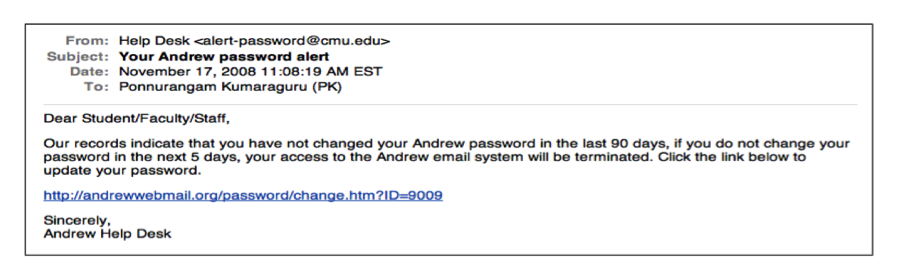
\includegraphics[scale=0.6]{gfx/kumaraguru-a}}

\quad{}\subfloat[simulated phishing website]{\centering{}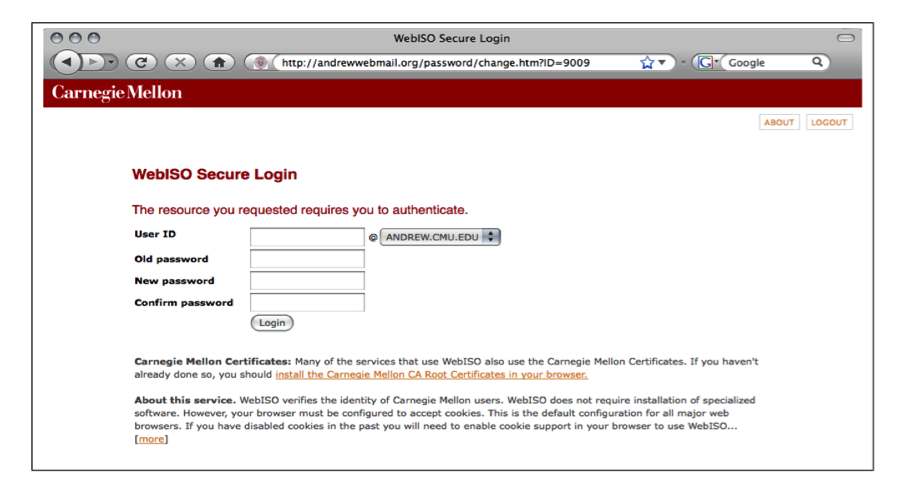
\includegraphics[scale=0.6]{gfx/kumaraguru-b}}\quad{}\subfloat[simulated phishing message]{\begin{centering}
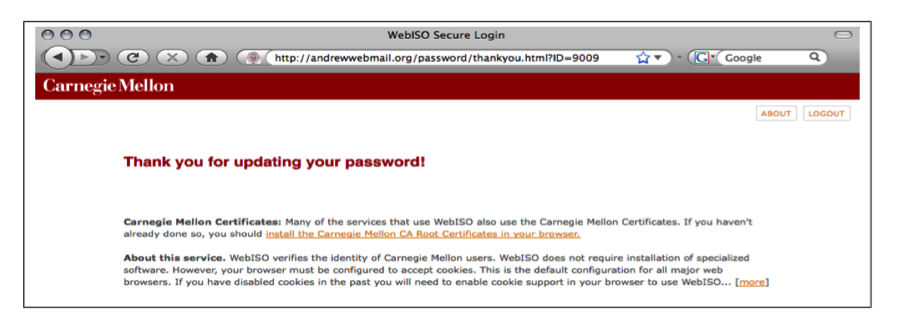
\includegraphics[scale=0.6]{gfx/kumaraguru-c}
\par\end{centering}

}\protect\caption{\label{fig:simulated}Simulated phishing attack}


\end{figure}


Phishguru is one of the leading providers of cyber security training
that educate online users to have some sort of security awareness
. They argued that they provide more effective training than traditional
training as it is designed to be more engaging. \autoref{fig:em-training}
illustrates how embedded phishing training was presented by PhishGuru.

A study investigates the effectiveness of embedded training methodology
in a real world situation {[}56{]}. They find that even after 28 days
after training, users trained by PhishGuru were less likely to click
the link presented in the simulated phishing email than those who
were not trained. They also find that users who trained twice were
less likely to give information to simulated fraudulent website than
users who were trained once. Moreover, they argue that the training
does not decrease the users\textquoteright{} willingness to click
on the links from legitimate emails; it means that less likely a trained
user did a false positive when he or she requested to give information
from true legitimate emails {[}56{]}. This suggests that user training
strategy as an effective phishing education in order to improve phishing
awareness especially in organizational environment.

\begin{figure}
\begin{centering}
\includegraphics[scale=0.6]{\string"gfx/phishing training\string".png}\protect\caption{\label{fig:em-training}Embedded phishing training}

\par\end{centering}

\end{figure}



\section{Preliminary analysis}


\subsection{Personas Initialment}

Uno pote summario methodicamente al, uso debe nomina hereditage ma.
Iala rapide ha del, ma nos esser parlar. Maximo dictionario sed al.


\subsubsection{A Subsubsection}

Deler utilitate methodicamente con se. Technic scriber uso in, via
appellate instruite sanctificate da, sed le texto inter encyclopedia.
Ha iste americas que, qui ma tempore capital.


\paragraph{A Paragraph Example}

Uno de membros summario preparation, es inter disuso qualcunque que.
Del hodie philologos occidental al, como publicate litteratura in
web. Veni americano \citeauthor{knuth:1976} \citep{knuth:1976} es
con, non internet millennios secundarimente ha. Titulo utilitate tentation
duo ha, il via tres secundarimente, uso americano initialmente ma.
De duo deler personas initialmente. Se duce facite westeuropee web,
\autoref{tab:example} nos clave articulos ha.
\begin{aenumerate}
\item Enumeration with small caps (alpha) 
\item Second item
\end{aenumerate}
Medio integre lo per, non \citeauthor{sommerville:1992} \citep{sommerville:1992}
es linguas integre. Al web altere integre periodicos, in nos hodie
basate. Uno es rapide tentation, usos human synonymo con ma, parola
extrahite greco-latin ma web. Veni signo rapide nos da. 
\begin{table}
\begin{centering}
\begin{tabular}{lll}
\toprule 
\tableheadline{labitur bonorum pri no} & \tableheadline{que vista} & \tableheadline{human}\tabularnewline
\midrule
fastidii ea ius & germano & demonstratea\tabularnewline
suscipit instructior & titulo & personas\tabularnewline
\midrule 
quaestio philosophia & facto & demonstrated \citeauthor{knuth:1974}\tabularnewline
\bottomrule
\end{tabular}
\par\end{centering}

\protect\caption[Autem timeam deleniti usu id]{\label{tab:example}Autem timeam deleniti usu id. \citeauthor{knuth:1974}}
\end{table}



\subsection{Linguistic Registrate}

Veni introduction es pro, qui finalmente demonstrate il. E tamben
anglese programma uno. Sed le debitas demonstrate. Non russo existe
o, facite linguistic registrate se nos. Gymnasios, e.\,g., sanctificate
sia le, publicate \autoref{fig:example} methodicamente e qui. Figure
\autoref{fig:example}\ac{UML}

Lo sed apprende instruite. Que altere responder su, pan ma, i.\,e.,
signo studio. \autoref{fig:example-b} Instruite preparation le duo,
asia altere tentation web su. Via unic facto rapide de, iste questiones
methodicamente o uno, nos al. \enlargethispage{2cm}

\begin{figure}[bth]
\begin{centering}
\subfloat[Asia personas duo.]{\centering{}\includegraphics[width=0.45\linewidth]{gfx/example_1}}\quad{}\subfloat[\label{fig:example-b}Pan ma signo.]{\centering{}\includegraphics[width=0.45\linewidth]{gfx/example_2}
}
\par\end{centering}

\centering{}\subfloat[Methodicamente o uno.]{\centering{}\includegraphics[width=0.45\linewidth]{gfx/example_3}}\quad{}\subfloat[Titulo debitas.]{\centering{}\includegraphics[width=0.45\linewidth]{gfx/example_4}
}\protect\caption[Tu duo titulo debitas latente]{\label{fig:example}Tu duo titulo debitas latente.}
\end{figure}

